\part{Práctica 1}
\section{Actividad 1-1}\label{p11}
\begin{center}
    \parbox{12cm}{\justify\textit{
        Elija 3 bases de datos de la UCI Machine Learning Repository de las que hay en Moodle y transformelas a .arff, indicando en cada una de ellas qué procedimiento ha seguido.
    }}
\end{center}

\subsection{Consideraciones generales}\label{ssc:consideraciones-generales}
Para la realización de la tarea he tomado la decisión de editar manualmente los archivos utilizando Visual Studio Code y guardarlos con la extensión \code{.arff}. El paso a csv utilizando excel que se ha sugerido en clase supone varios cambios de formato en los que pueden aparecer diversos problemas como conflictos entre el separador de columnas CSV y el separador de decimales o miles, problemas con el carácter de salto de línea, codificación, etc.

Para conocer los identificadores y tipos de los atributos de cada base de datos he consultado el archivo \code{.names} del directorio de descarga de cada base de datos, que contiene el listado de campos con su nombre, su tipo y sus posibles valores, si procede. He consultado la especificación del formato \code{.arff} en la \href{https://www.cs.waikato.ac.nz/ml/weka/arff.html}{página correspondiente del manual de weka}\footnote{\url{https://www.cs.waikato.ac.nz/ml/weka/arff.html}}. Como puede comprobarse en la figura \ref{fig:ejemplo-arff}, un archivo \code{.arff} consta de tres secciones:
\begin{figure}[ht]
    \centering
    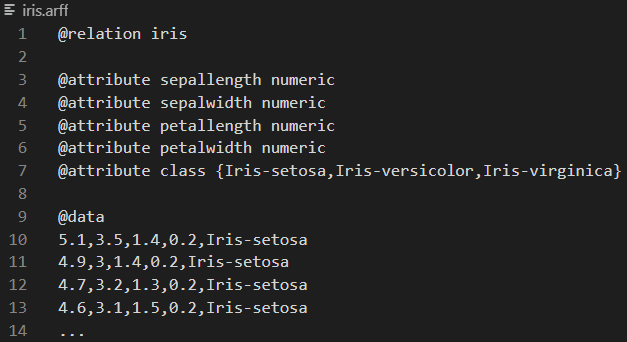
\includegraphics[scale=0.6]{ejemplo-archivo-arff}
    \caption{Ejemplo de archivo \code{.arff}}
    \label{fig:ejemplo-arff}
\end{figure}
\begin{enumerate}
    \item Identificación de la base de datos. Se trata de una línea con el token \code{@relation} seguido por un espacio y el nombre de la base de datos. Por ejemplo: \code{@relation breast-cancer}.
    \item Identificación de los atributos. Tantas líneas como atributos tenga la base de datos, cada una comienza con el token \code{@atribute} seguido del nombre del atributo y el tipo. Los tipos pueden ser:
        \begin{itemize}
            \item Numéricos: \code{@attribute <nombre\string_atributo>\space numeric}
            \item Cadenas de texto: \code{@attribute <nombre\string_atributo> \space string}
            \item Listas de etiquetas: \code{@attribute <nombre\string_atributo> \space\string{valor\string_1, valor\string_2, \dots\string}}
            \item Fechas: \code{@attribute <nombre\string_atributo>\space date [formato\string_de\string_fecha]}. El formato de fecha es opcional, y por defecto acepta ISO-8601 y ``yyyy-MM-dd'T'HH:mm:ss''.
        \end{itemize}
    \item Bloque de datos. Esta sección se inicia con una línea que contiene únicamente palabra clave \code{@data}. A continuación se encontrarán los registros dispuestos en líneas y con sus atributos separados por comas, en el mismo orden en que se han especificado en la cabecera:
    \begin{center}
        \parbox{5.1cm}{\code{@data \\
            v1a1, v1a2, \dots, v1aN \\
            v2a1, v2a2, \dots, v2aN \\
            \dots \\
            vMa1, vMa2, \dots, vMaN
        }}
    \end{center}

\end{enumerate}

\subsection{Base de datos \code{breast-cancer}}
Tras aplicar el tratamiento mencionado en el apartado \ref{ssc:consideraciones-generales} al archivo \code{breast-cancer.data} se ha obtenido el fichero \code{.arff} (fig. \ref{fig:breast-cancer-arff}) y una vez cargado en Weka (fig. \ref{fig:breast-cancer-weka}) y se han obtenido las siguientes conclusiones:

\begin{enumerate}
    \item La base de datos tiene 10 atributos, de los cuales el primero es la clase, que toma los valores ``no-recurrence-events'' y ``recurrence-events''. Convendría colocar la clase al final, que es su lugar por defecto.
    \item Los atributos son nominales basados en etiquetas (por ejemplo breast\_quad, menopause\dots) o en rangos numéricos (inv\_nodes, tumor\_size\dots). El atributo deg\_malig se podría poner como numérico ya que parece representar el grado de malignidad en un rango de 1 a 3, por lo que hay una distancia distinta entre los elementos (por ejemplo 1-2 y 1-3).
\end{enumerate}

\begin{figure}[H]
    \centering
    \begin{minipage}{0.49\textwidth}
        \centering
        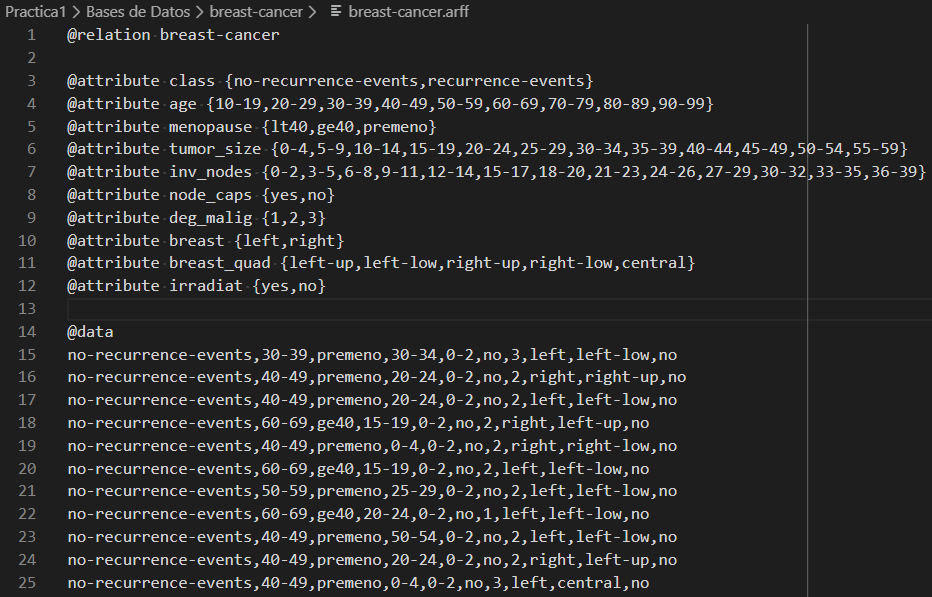
\includegraphics[scale=0.3]{breast-cancer-arff}
        \caption{Captura de \code{breast-cancer.arff}.}
        \label{fig:breast-cancer-arff}
    \end{minipage}
    \begin{minipage}{0.49\textwidth}
        \centering
        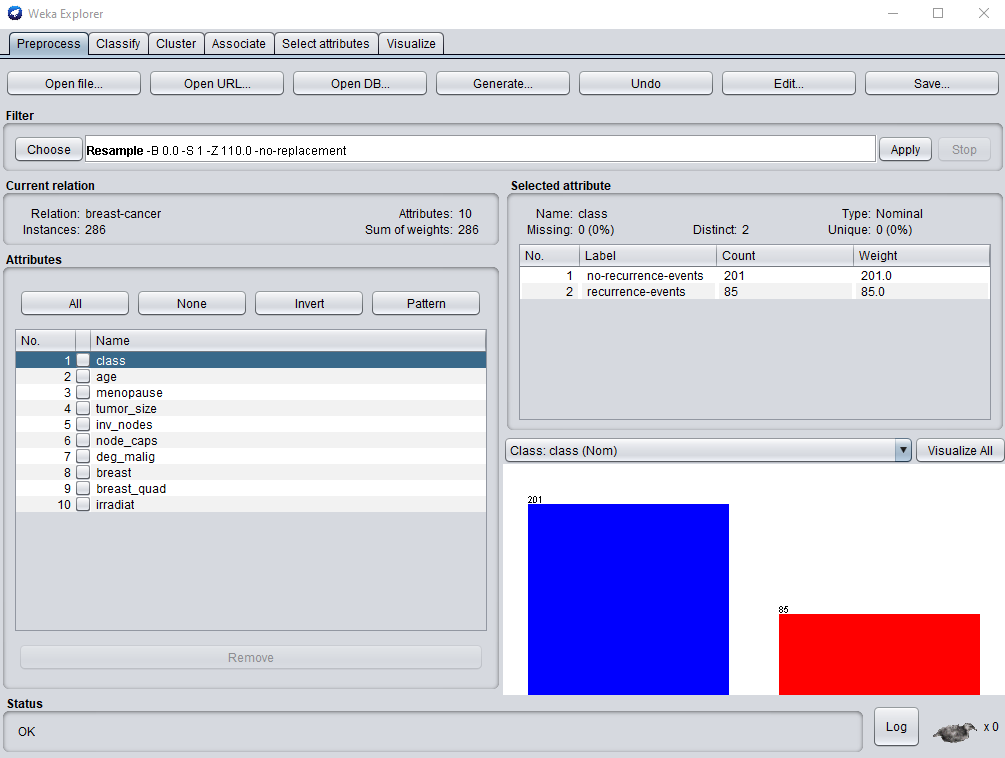
\includegraphics[scale=0.29]{breast-cancer-weka}
        \caption{Archivo \code{breast-cancer.arff} cargado en Weka.}
        \label{fig:breast-cancer-weka}
    \end{minipage}
\end{figure}

\subsection{Base de datos \code{dermatology}}
Tras aplicar el tratamiento mencionado en el apartado \ref{ssc:consideraciones-generales} al archivo \code{dermatology.data} se ha obtenido el fichero \code{.arff} (fig. \ref{fig:dermatology-arff}) y una vez cargado en Weka (fig. \ref{fig:dermatology-weka}) y se han obtenido las siguientes conclusiones:

\begin{enumerate}
    \item La base de datos tiene 34 atributos independientes y una clase. En total hay 366 patrones.
    \item La mayoría los atributos son de tipo numérico con valores [0-3]. En la descripción se indica que los valores indican un grado obtenido de un análisis. El caso del atributo family-history es una excepción, ya que es nominal con valores 0 y 1 y representa si alguna de las enfermedades ha sido observada en la familia. Otra excepción es la edad, que siendo numérica, no está restringida al rango anterior.
    \item La clase toma valores de 1 a 6 y cada valor representa un diagnóstico diferente, por lo que es un dato nominal.
\end{enumerate}
\begin{figure}[H]
    \centering
    \begin{minipage}{0.45\textwidth}
        \centering
        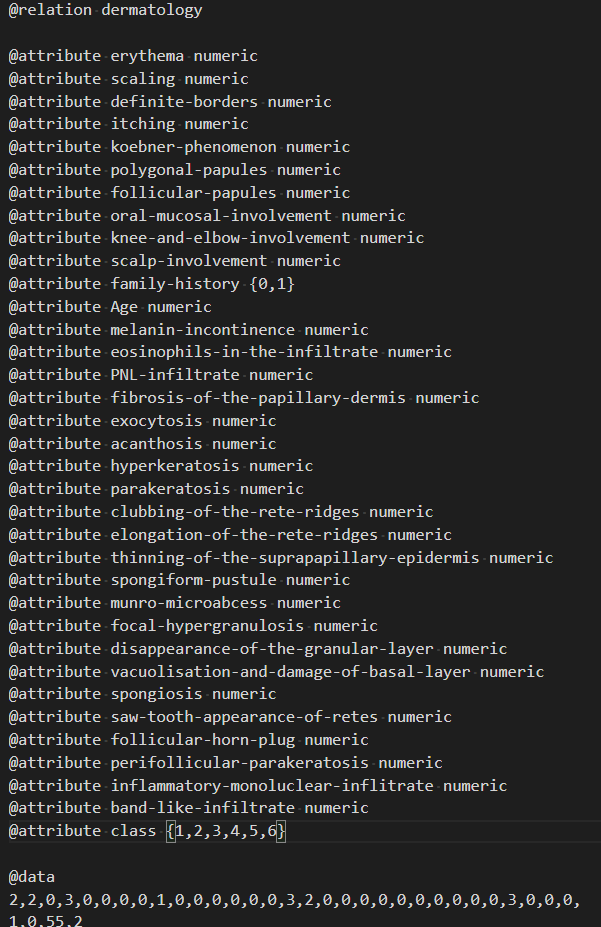
\includegraphics[scale=0.40]{dermatology-arff}
        \caption{Captura de \code{dermatology.arff}.}
        \label{fig:dermatology-arff}
    \end{minipage}\hfill
    \begin{minipage}{0.55\textwidth}
        \centering
        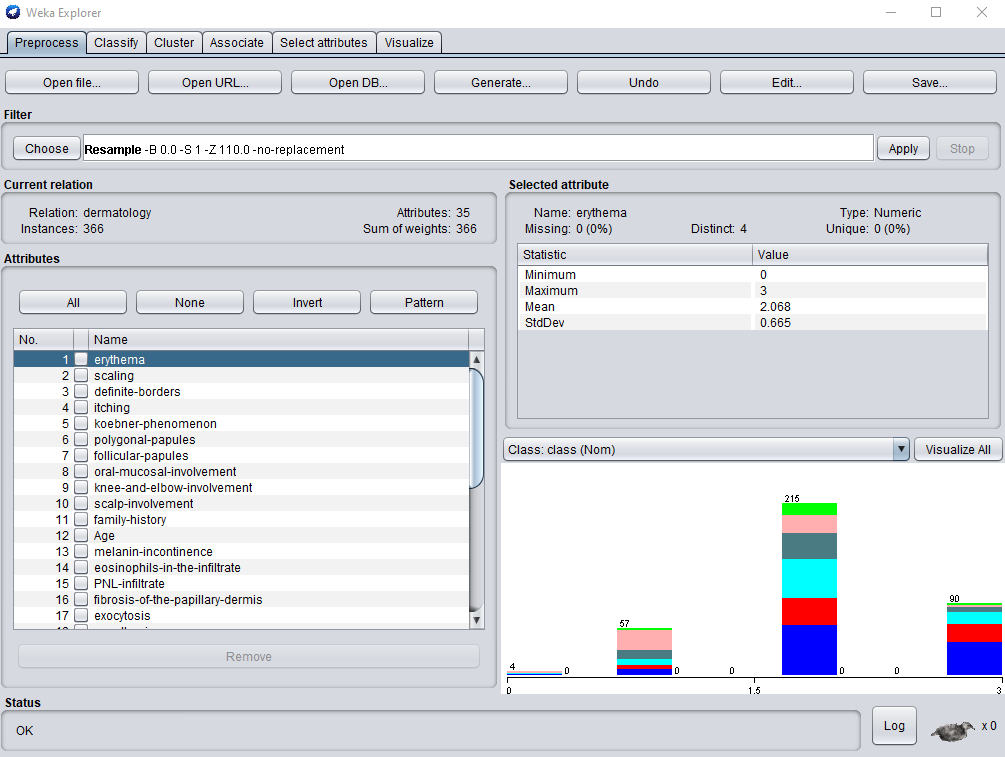
\includegraphics[scale=0.33]{dermatology-weka}
        \caption{Archivo \code{dermatology.arff} cargado en Weka.}
        \label{fig:dermatology-weka}
    \end{minipage}
\end{figure}


\subsection{Base de datos \code{wine}}
Tras aplicar el tratamiento mencionado en el apartado \ref{ssc:consideraciones-generales} al archivo \code{wine.data} se ha obtenido el fichero \code{.arff} (fig. \ref{fig:wine-arff}) y una vez cargado en Weka (fig. \ref{fig:wine-weka}) y se han obtenido las siguientes conclusiones:

\begin{enumerate}
\item La base de datos tiene 13 atributos independientes y una clase al principio.
\item Los atributos son numéricos continuos.
\item La clase toma valores 1, 2 o 3 con frecuencias 59, 71 y 48 respectivamente. Es un dato nominal
\end{enumerate}


\begin{figure}[H]
    \centering
    \begin{minipage}{0.49\textwidth}
        \centering
        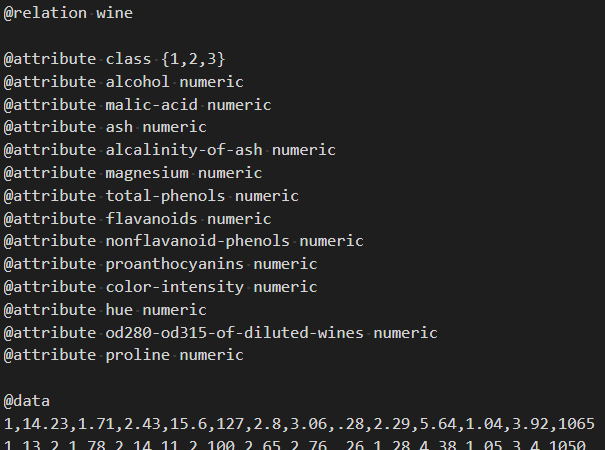
\includegraphics[scale=0.45]{wine-arff}
        \caption{Captura del archivo \code{wine.arff}.}
        \label{fig:wine-arff}
    \end{minipage}
    \begin{minipage}{0.49\textwidth}
        \centering
        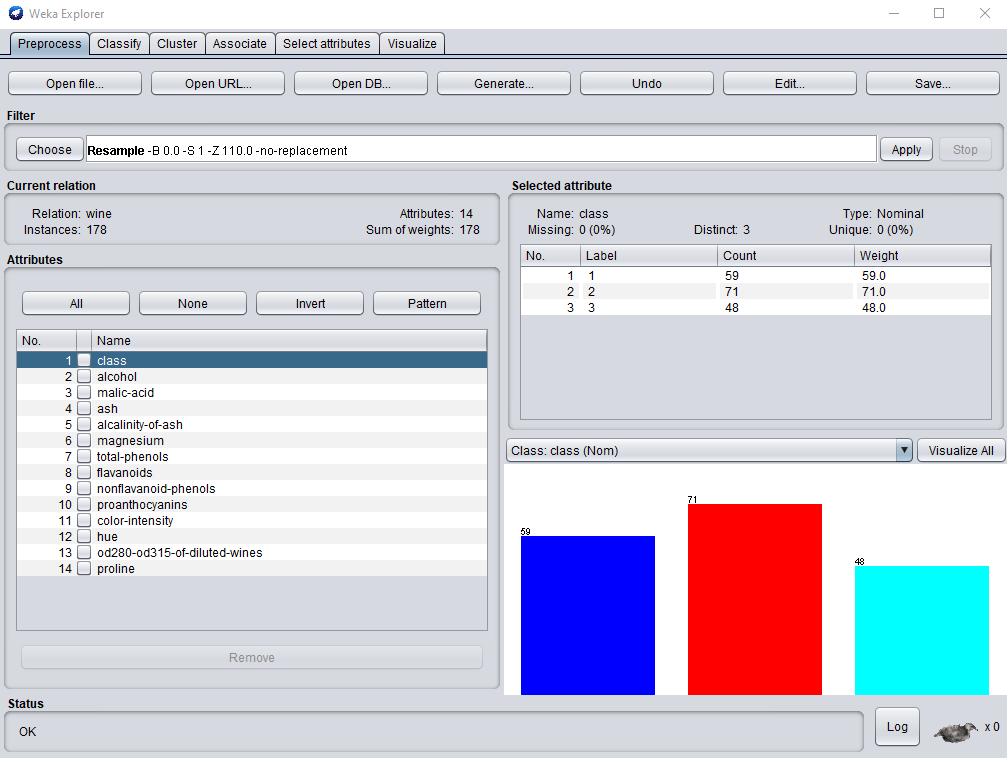
\includegraphics[scale=0.29]{wine-weka}
        \caption{Archivo \code{wine.arff} cargado en Weka.}
        \label{fig:wine-weka}
    \end{minipage}
\end{figure}


%-------------------------------------------------------------------------------
%-------------------------------------------------------------------------------
%-------------------------------------------------------------------------------
\clearpage
\section{Actividad 1-2}\label{p12}
\begin{center}
    \parbox{12cm}{\justify\textit{Elija 3 filtros No Supervisados de los que aparecen listados, expliquelos y describa cómo quedan los datos antes y después al aplicarlos sobre una o varias bases de datos.
    \begin{itemize}
        \item Consulte el UCI Machine Learning Repository para una descripción de la base de datos y la transformación a \code{.arff}
        \item Si no puede aplicar un filtro elegido en ninguna base de datos describa por qué, y constrúyase una base de datos ficticia y pequeña donde si pueda aplicarlo.
        \item Use capturas de pantalla, salidas de Weka y todo lo que considere necesario para sus ejercicios.
        \item La puntuación variará en función de la argumentación y dificultad de los filtros elegidos.
        \begin{enumerate}
            \item filters/unsupervised/attribute/Normalize
            \item filters/unsupervised/attribute/ReplaceMissingValues
            \item filters/unsupervised/attributes/NominalToBinary
            \item filters/unsupervised/intance/RemoveDuplicates
            \item filters/unsupervised/instance/Resample
            \item filters/unsupervised/attribute/Remove
            \item filters/unsupervised/attributes/RemoveUseless
        \end{enumerate}
    \end{itemize}
    }}
\end{center}

\subsection{filters/unsupervised/instance/Resample}
\label{ssc:unsupervised-resample}
Según la información que proporciona Weka, este filtro produce un conjunto de datos mediante un remuestreo de la base de datos original. Este remuestreo no supervisado se utiliza para aumentar el número de patrones (\textbf{oversampling}) mediante la creación de duplicados de patrones existentes o para reducirlo (\textbf{undersampling}) mediante la eliminación de patrones aleatorios. La selección de patrones para oversampling se puede hacer con o sin repetición. Si es sin repetición, un patrón duplicado no podrá ser seleccionado de nuevo para su duplicación.

Para ilustrar el comportamiento del filtro observaremos cómo cambian las frecuencias relativas en las clases tras realizar diversos undersamplings y oversamplings. La hipótesis es que las frecuencias relativas no se mantendrán constantes ya que el filtro elimina o duplica patrones al azar. En Weka, se ha cargado la base de datos \code{dermatology.arff}. En la base de datos hay inicialmente 366 patrones repartidos en 6 clases con las frecuencias que se pueden ver en la columna ``Frec. Orig.'' del cuadro \ref{tab:unsupervised-resample-undersample-dist}. Posteriormente, se ha seleccionado el filtro Resample no supervisado: \code{unsupervised/instance/Resample}.

El filtro Resample no supervisado cuenta con los siguientes parámetros de configuración (ver fig. \ref{fig:unsupervised-resample}):

\begin{itemize}
    \item \code{invertSelection False/True}: Invierte la selección (descartados por seleccionados).
    \item \code{noReplacement True/False}: Deshabilita el reemplazo de instancias, esto es, al seleccionar instancias para duplicar, permite o no que la misma instancia sea seleccionada más de una vez. Esto sólo tiene sentido al hacer oversampling (sampleSizePercent>100).
    \item \code{randomSeed (núm 1)}: Semilla para la selección aleatoria.
    \item \code{sampleSizePercent (núm 100)}: Tamaño del conjunto resultante como \% del original.
\end{itemize}

\begin{figure}[ht]
    \centering
    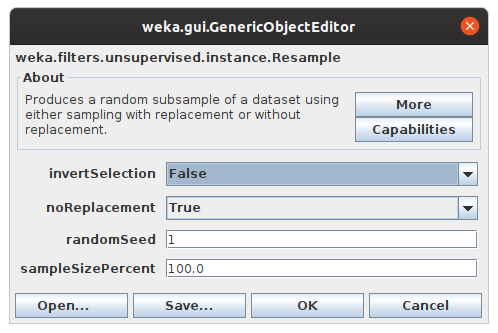
\includegraphics[scale=0.35]{unsupervised-resample}
    \caption{Configuración del filtro \code{unsupervised/Resmaple}.}
    \label{fig:unsupervised-resample}
\end{figure}

Para este ejercicio se han establecido los siguientes valores de configuración:
\begin {itemize}
    \item \code{randomSeed=50}
    \item \code{noReplacement=True}
    \item \code{invertSelection=False}
    \item \code{sampleSizePercent=\{75, 50, 25\}}.
\end{itemize}

En el cuadro \ref{tab:unsupervised-resample-undersample-dist} y figura \ref{fig:unsupervised-resample-undersample-dist} se muestra la distribución de las clases al utilizar el filtro para realizar \textbf{undersampling} reduciendo el conjunto al 75\%, al 50\% y al 25\%. Cada resample se ha realizado sobre el conjunto original. El proceso ha sido: aplicar el filtro, tomar los datos, deshacer, siguiente.
\begin{table}[ht]
    \centering
    \begin{tabular}{|r|rr|rr|rr|rr|}
        \hline
        \multicolumn{1}{|l|}{Clase} & \multicolumn{2}{r|}{Frec. Orig.} & \multicolumn{2}{r|}{Frec. US75} & \multicolumn{2}{r|}{Frec. US50} & \multicolumn{2}{r|}{Frec. US25} \\ 
        \hline
        1 & 112 & 30,60\% & 87 & 31,75\% & 62 & 33,88\% & 31 & 34,07\% \\
        2 & 61  & 16,67\% & 43 & 15,69\% & 25 & 13,66\% & 13 & 14,29\% \\
        3 & 72  & 19,67\% & 54 & 19,71\% & 37 & 20,22\% & 16 & 17,58\% \\
        4 & 49  & 13,39\% & 37 & 13,50\% & 24 & 13,11\% & 12 & 13,19\% \\
        5 & 52  & 14,21\% & 39 & 14,23\% & 27 & 14,75\% & 16 & 17,58\% \\
        6 & 20  & 5,46\%  & 14 & 5,11\%  & 8  & 4,37\%  & 3  & 3,30\%  \\
        \hline 
        Total\footnote{Porcentajes respecto al tamaño número inicial de patrones} & 366 & 100\% & 274 & 74,86\% & 183 & 50,00\% & 91 & 24,86\% \\
        \hline
    \end{tabular}
    \caption{Frecuencias de clases con diferentes undersamplings}
    \label{tab:unsupervised-resample-undersample-dist}
\end{table}
\begin{figure}[H]
    \centering
    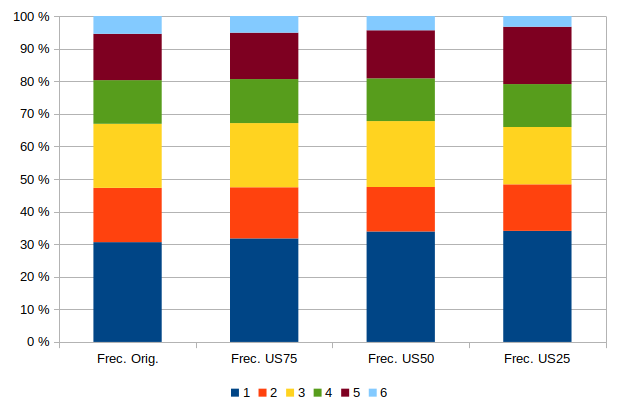
\includegraphics[scale=0.45]{unsupervised-resample-undersample-dist}
    \caption{Frecuencias de clases con diferentes undersamplings}
    \label{fig:unsupervised-resample-undersample-dist}
\end{figure}

Siguiendo la misma dinámica que con el undersampling, se ha realizado un oversampling del conjunto original utilizando el filtro Resample no supervisado, observado que sólo tiene efecto cuando el parámetro \code{noReplacement} se pone a valor \code{False}. En el cuadro \ref{tab:unsupervised-resample-oversample-dist} y figura \ref{fig:unsupervised-resample-oversample-dist} se pueden ver las frecuencias de las diferentes clases al realizar oversamplings al 125\%, 150\%, 175\% y 200\%.

\begin{table}[ht]
    \centering
    \begin{tabular}{|r|rr|rr|rr|rr|rr|}
        \hline
        \multicolumn{1}{|c|}{Clase} & \multicolumn{2}{c|}{Frec. Orig.} & \multicolumn{2}{c|}{Frec. OS125} & \multicolumn{2}{c|}{Frec. OS150} & \multicolumn{2}{c|}{Frec. OS175} & \multicolumn{2}{c|}{Frec. OS200} \\ 
        \hline
        1 & 112 & 30,60\% & 136 & 29,76\% & 168 & 30,60\% & 190 & 29,69\% & 216 & 29,51\% \\
        2 & 61  & 16,67\% & 66  & 14,44\% & 83  & 15,12\% & 100 & 15,63\% & 114 & 15,57\% \\
        3 & 72  & 19,67\% & 89  & 19,47\% & 107 & 19,49\% & 127 & 19,84\% & 149 & 20,36\% \\
        4 & 49  & 13,39\% & 58  & 12,69\% & 68  & 12,39\% & 80  & 12,50\% & 88  & 12,02\% \\
        5 & 52  & 14,21\% & 79  & 17,29\% & 91  & 16,58\% & 104 & 16,25\% & 118 & 16,12\% \\
        6 & 20  & 5,46\%  & 29  & 6,35\%  & 32  & 5,83\%  & 39  & 6,09\%  & 47  & 6,42\%  \\
        \hline
        Total\footnote{Porcentajes respecto al tamaño muestral inicial} & 366 & 100,00 \% & 457 & 124,86 \% & 549          & 150,00 \% & 640 & 174,86 \% & 732 & 200,00 \% \\
        \hline
    \end{tabular}
    \caption{Frecuencias de clases con diferentes oversamplings}
    \label{tab:unsupervised-resample-oversample-dist}
\end{table}
\begin{figure}[ht]
    \centering
    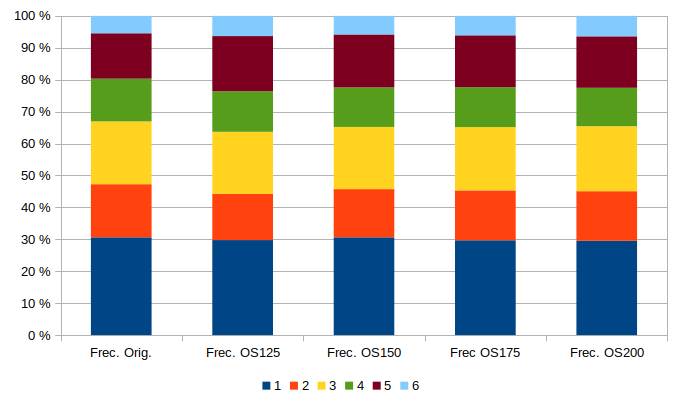
\includegraphics[scale=0.45]{unsupervised-resample-oversample-dist}
    \caption{Frecuencias de clases con diferentes oversamplings}
    \label{fig:unsupervised-resample-oversample-dist}
\end{figure}

Al comparar la frecuencia de cada clase tras las distintas aplicaciones del filtro (fig. \ref{fig:unsupervised-resample-undersample-dist} y \ref{fig:unsupervised-resample-oversample-dist}), se puede observar que varían para los distintos valores de \code{sampleSizePercent}, aunque no demasiado. Dado que se trata de un filtro no supervisado (no tiene en cuenta la clase a la hora de eliminar o crear patrones), este hecho puede deberse a que la base de datos es bastante homogénea en el sentido de que los patrones de cada clase se encuentran distribuidos regularmente a lo largo de la base de datos. En casos de undersampling extremo (ej.: reducción al 4\%) se observa cómo llegan a desaparecer todos los patrones de algunas clases.

En el apartado \ref{ssc:supervised-resample} se probará el filtro supervisado equivalente para comparar las frecuencias obtenidas. Sería lógico suponer que en el filtro supervisado, las frecuencias relativas de las clases variarán menos que en el supervisado según se va reduciendo la muestra.

\subsection{filters/unsupervised/attributes/NominalToBinary}
El filtro no supervisado NominalToBinary reemplaza cada atributo nominal que tenga más de dos valores distintos, por tantos atributos binarios como valores diferentes tenga el atributo original. Estos atributos binarios tendrán valor 1 si el patrón tenía el valor correspondiente al atributo binario en el atributo original y 0 si no. Este proceso se denomina binarización.

\begin{figure}[ht]
    \centering
    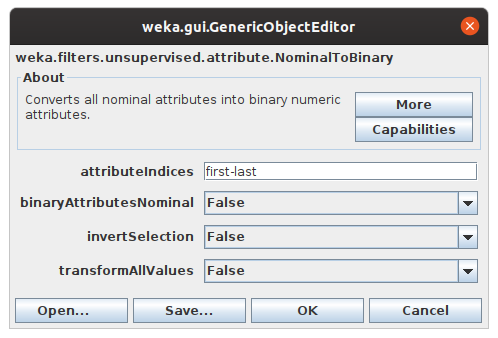
\includegraphics[scale=0.36]{unsupervised-nominal-to-binary}
    \caption{Configuración del filtro \code{unsupervised/NominalToBinary}.}
    \label{fig:unsupervised-nominal-to-binary}
\end{figure}

El filtro NominalToBinary, cuyo formulario de configuración puede verse en la figura \ref{fig:unsupervised-nominal-to-binary} cuenta con los siguientes parámetros:

\begin{itemize}
    \item \code{attributeIndices ([first-last])}: indica el rango de atributos que se van a binarizar. Se especifican los índices o rangos de índices separados por comas. También son válidos los valores ``first'' y ``last''.
    \item \code{binaryAttributesNominal False/True}: Permite establecer si los valores de los nuevos atributos binarios serán valores de tipo 0-1 o si o nominal f-t.
    \item \code{invertSelection False/True}: Si es False, se binarizan los atributos indicados en attributeIndices. Si es True, se binarizan sólo los que no están especificados en dicho parámetro.
    \item \code{transformAllValues False/True}: Si es True, se procesan también los atributos nominales con sólo dos valores.
\end{itemize}

Para ilustrar el funcionamiento de este filtro se ha cargado la base de datos \code{breast-cancer.arff} en Weka y se ha aplicado el filtro a los campos 3 y 6. El primero es nominal con tres valores y el segundo es nominal con dos valores (fig. \ref{fig:breast-cancer-attribute-menopause} y \ref{fig:breast-cancer-attribute-node-caps}). La configuración del filtro es \code{attributeIndices=3,6}, \code{binaryAttributesNominal=True}, \code{invertSelection=False} y \code{transformAllValues=False}, por lo tanto se espera que reemplace el atributo \code{menopause} por tres atributos, uno por cada uno de los tres valores que toma, y que el atributo \code{code\_caps} se quede intacto ya que salvo que se ponga \code{transformAllValues=True} o \code{binaryAttributesNominal=False}, este filtro no altera los atributos nominales de dos valores.

\begin{figure}[ht]
    \centering
    \begin{minipage}{0.50\textwidth}
        \centering
        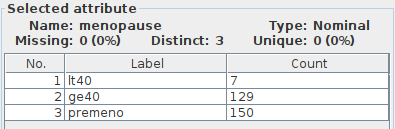
\includegraphics[scale=0.55]{breast-cancer-attribute-menopause}
        \caption{Información del atributo \code{menopause}}
        \label{fig:breast-cancer-attribute-menopause}
    \end{minipage}\hfill
    \begin{minipage}{0.50\textwidth}
        \centering
        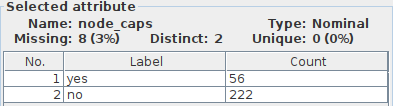
\includegraphics[scale=0.52]{breast-cancer-attribute-node-caps}
        \caption{Información del atributo \code{node\_caps}}
        \label{fig:breast-cancer-attribute-node-caps}
    \end{minipage}
\end{figure}

Los resultados obtenidos (fig. \ref{fig:breast-cancer-nominal-to-binary-1}) confirman la hipótesis:
\begin{itemize}
    \item El filtro ha reemplazado el atributo \code{menopause} por tres campos binarios, uno por cada valor diferente que tomaba el atributo original: \code{menopause=lt40}, \code{menopause=ge40} y \code{menopause=premeno}.
    \item El filtro no ha alterado el atributo \code{node\_caps} porque sólo toma dos valores diferentes.
    \item Las distribuciones de los nuevos campos son coherentes con la distribución del campo original, es decir: hay 7 patrones con valor 1 en \code{menopause=lt40}, hay 129 patrones con valor 1 en \code{menopause=ge40} y hay 150 patrones con valor 1 en \code{menopause=premeno}.
\end{itemize}

\begin{figure}[ht]
    \centering
    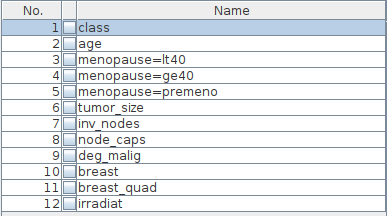
\includegraphics[scale=0.5]{breast-cancer-nominal-to-binary-1}
    \caption{Campos tras aplicar \code{NominalToBinary}.}
    \label{fig:breast-cancer-nominal-to-binary-1}
\end{figure}

Se ha observado que si se establece a False el parámetro \code{}, altera los atributos nominales con dos valores, reemplazando los valores nominales por 0 y 1 pero sin reemplazar el atributo. Para que reemplace el atributo como hace con los nominales de más de dos valores, debe ponerse a True el parámetro \code{transformAllValues}.

\subsection{filters/unsupervised/attributes/RemoveUseless}
El filtro no supervisado RemoveUseless elimina los atributos de la base de datos que no varían o que lo hacen demasiado. Es decir, elimina todos los atributos con valor constante o cuya variación excede el porcentaje indicado en el parámetro \code{maximumVariancePercentageAllowed}. Para calcular la variación de un atributo se aplica la siguiente fórmula:
\begin{equation*}
\text{Variación}=\dfrac{\text{Nº Valores Distintos}}{\text{Nº Valores Total}}\cdot100
\end{equation*}

El formulario de configuración de este filtro puede verse en la figura \ref{fig:unsupervised-remove-useless}.

\begin{figure}[ht]
    \centering
    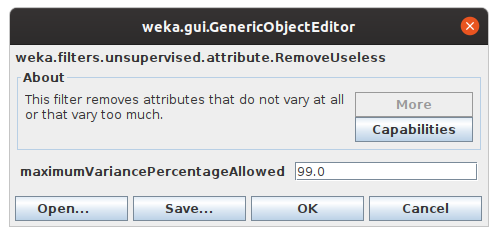
\includegraphics[scale=0.5]{unsupervised-remove-useless}
    \caption{Configuración del filtro \code{unsupervised/RemoveUseless}}
    \label{fig:unsupervised-remove-useless}
\end{figure}

Para probar este filtro se va a componer una base de datos de ejemplo con 200 patrones y 6 atributos más una clase. Los atributos tienen las siguientes características:
\begin{enumerate}
    \item \code{atr1} nominal binario con valores SI/NO. Todos los patrones tienen valor NO. Los datos que arroja Weka sobre este atributo se ven en la fig. \ref{fig:unsupervised-remove-useless-atr1}.
    \item \code{atr2} nominal binario con valores SI/NO. Todos los patrones tienen valor NO excepto uno con valor SI. Este atributo se ha puesto como control del primero, para comprobar que no es eliminado por el filtro. Los datos que arroja Weka sobre este atributo se ven en la fig. \ref{fig:unsupervised-remove-useless-atr2}.    
    \item \code{atr3} numérico. Todos los patrones tienen valor 7.0. Es el mismo caso que \code{atr1} para numérico. Se espera que el filtro elimine este campo también. Los datos que arroja Weka sobre este atributo se ven en la fig. \ref{fig:unsupervised-remove-useless-atr3}.
    \item \code{atr4} nominal con valores \code{a1\dots a200}. Cada atributo toma un valor diferente. La tasa de variación es $\frac{200}{200}\cdot100=100$. Los datos que arroja Weka sobre este atributo se ven en la fig. \ref{fig:unsupervised-remove-useless-atr3}.
    \item \code{atr5} nominal con valores \code{b1\dots b199}. Cada atributo toma un valor diferente salvo los dos últimos que son iguales. La tasa de variación es $\frac{199}{200}\cdot100=99,5$. Los datos que arroja Weka sobre este atributo se ven en la fig. \ref{fig:unsupervised-remove-useless-atr5}.
    \item \code{atr6} nominal con valores \code{a1\dots a200}. Cada atributo toma un valor diferente salvo los tres últimos que son iguales. La tasa de variación es $\frac{198}{200}\cdot100=99$. Los datos que arroja Weka sobre este atributo se ven en la fig. \ref{fig:unsupervised-remove-useless-atr6}.
\end{enumerate}

\begin{figure}[H]
    \centering
    \begin{minipage}{0.50\textwidth}
        \centering
        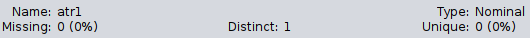
\includegraphics[scale=0.4]{unsupervised-remove-useless-attr1}
        \caption{Atributo \code{atr1}}
        \label{fig:unsupervised-remove-useless-atr1}
    \end{minipage}\hfill
    \begin{minipage}{0.50\textwidth}
        \centering
        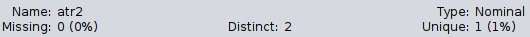
\includegraphics[scale=0.4]{unsupervised-remove-useless-attr2}
        \caption{Atributo \code{atr2}}
        \label{fig:unsupervised-remove-useless-atr2}
    \end{minipage}
\end{figure}
\begin{figure}[H]
    \centering
    \begin{minipage}{0.50\textwidth}
        \centering
        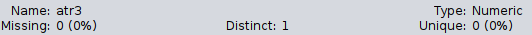
\includegraphics[scale=0.4]{unsupervised-remove-useless-attr3}
        \caption{Atributo \code{atr3}}
        \label{fig:unsupervised-remove-useless-atr3}
    \end{minipage}\hfill
    \begin{minipage}{0.50\textwidth}
        \centering
        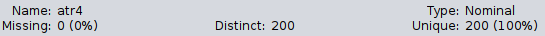
\includegraphics[scale=0.4]{unsupervised-remove-useless-attr4}
        \caption{Atributo \code{atr4}}
        \label{fig:unsupervised-remove-useless-atr4}
    \end{minipage}
\end{figure}
\begin{figure}[H]
    \centering
    \begin{minipage}{0.50\textwidth}
        \centering
        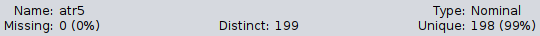
\includegraphics[scale=0.4]{unsupervised-remove-useless-attr5}
        \caption{Atributo \code{atr5}}
        \label{fig:unsupervised-remove-useless-atr5}
    \end{minipage}\hfill
    \begin{minipage}{0.50\textwidth}
        \centering
        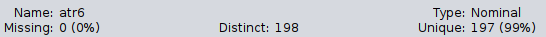
\includegraphics[scale=0.4]{unsupervised-remove-useless-attr6}
        \caption{Atributo \code{atr6}}
        \label{fig:unsupervised-remove-useless-atr6}
    \end{minipage}
\end{figure}

Se aplicará la configuración por defecto del filtro, que especifica el valor 99 para el parámetro \code{maximumVaiancePercentajeAllowed}. Se espera que el filtro elimine los atributos 1 y 3 por ser constantes y 4 y 5 por tener una tasa de variación superior al 99\% configurado en el parámetro. Como se puede comprobar en la figura \ref{fig:unsupervised-remove-useless-aplicado}, el filtro se ha comportado como se esperaba: eliminando los atributos \code{atr1}, \code{atr3}, \code{atr4} y \code{atr5} y manteniendo \code{atr2} y \code{atr6}.

\begin{figure}[H]
    \centering
    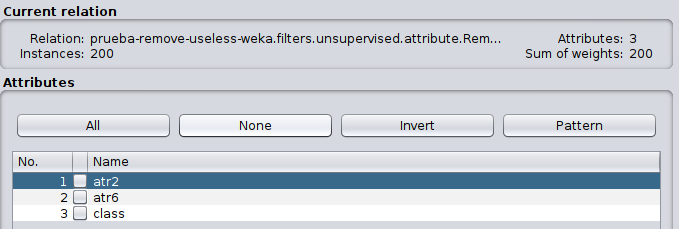
\includegraphics[scale=0.5]{unsupervised-remove-useless-aplicado}
    \caption{Resultado de aplicar el filtro \code{RemoveUseless}.}
    \label{fig:unsupervised-remove-useless-aplicado}
\end{figure}

%-------------------------------------------------------------------------------
%-------------------------------------------------------------------------------
%-------------------------------------------------------------------------------
\clearpage
\section{Actividad 1-3}\label{p13}
\begin{center}
    \parbox{12cm}{\justify\textit{Elija 3 filtros Supervisados de los que aparecen listados, expliquelos y describa cómo quedan los datos antes y después al aplicarlos sobre una o varias bases de datos.
    \begin{itemize}
        \item Consulte el UCI Machine Learning Repository para una descripción de la base de datos y la transformación a \code{.arff}
        \item Si no puede aplicar un filtro elegido en ninguna base de datos describa por qué, y constrúyase una base de datos ficticia y pequeña donde si pueda aplicarlo.
        \item Use capturas de pantalla, salidas de Weka y todo lo que considere necesario para sus ejercicios.
        \item La puntuación variará en función de la argumentación y dificultad de los filtros elegidos.
        \begin{enumerate}
            \item filters/supervised/attribute/Discretize
            \item filters/supervised/attribute/NominalToBinary
            \item filters/supervised/instance/SpreadSubsample
            \item filters/supervised/instance/ClassBalancer
            \item filters/supervised/instance/Resample
        \end{enumerate}
    \end{itemize}
    }}
\end{center}


\subsection{filters/supervised/instance/Resample}
\label{ssc:supervised-resample}
El filtro Resample supervisado produce un conjunto de datos mediante un remuestreo de la base de datos original teniendo en cuenta la clase. Este remuestreo supervisado se utiliza para aumentar el número de patrones (\textbf{oversampling}) mediante la creación de duplicados de patrones existentes o para reducirlo (\textbf{undersampling}) mediante la eliminación de patrones manteniendo ciertas proporciones entre los patrones de cada clase. La selección de patrones para oversampling se puede hacer con o sin repetición. Si es sin repetición, un patrón duplicado no podrá ser seleccionado de nuevo para su duplicación. Según la documentación, la clase debe ser de tipo nominal para poder utilizar este filtro. De lo contrario, deberemos utilizar la versión no supervisada \ref{ssc:unsupervised-resample}.

Para comprobar el comportamiento del filtro observaremos cómo cambian las frecuencias relativas en las clases tras realizar diversos undersamplings y oversamplings en función del valor del parámetro \code{biasToUniformClass}. La hipótesis es que para el valor 0 la distribución de la clase se mantendrá igual mientras que para valor 1 se igualarán. Para valores intermedios del parámetro, mientras más cerca de 1, producirán un resultado más uniforme. En Weka, se ha cargado la base de datos \code{dermatology.arff}. En la base de datos hay inicialmente 366 patrones repartidos en 6 clases con las frecuencias que se pueden ver en la columna ``Frec. Orig.'' del cuadro \ref{tab:unsupervised-resample-oversample-dist}. Posteriormente, se ha seleccionado el filtro Resample supervisado: \code{supervised/instance/Resample} cuyo formulario de configuración se puede ver en la figura \ref{fig:supervised-resample}.

\begin{figure}[ht]
    \centering
    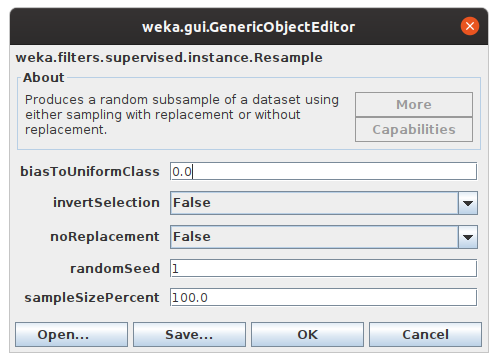
\includegraphics[scale=0.5]{supervised-resample}
    \caption{Configuración del filtro \code{supervised/Resmaple}.}
    \label{fig:supervised-resample}
\end{figure}
El filtro Resample supervisado cuenta con los siguientes parámetros:

\begin{itemize}
    \item \code{biasToUniformClass (núm [0.0-1.0])}: Establece el tipo de sesgo del remuestreo: para 0 se mantiene distribución original de la clase, para 1, la distribución es uniforme.
    \item \code{invertSelection False/True}: Invierte la selección (descartados por seleccionados).
    \item \code{noReplacement True/False}: Deshabilita el reemplazo de instancias, esto es, al seleccionar instancias para duplicar, permite o no que la misma instancia sea seleccionada más de una vez. Esto sólo tiene sentido al hacer oversampling (\code{sampleSizePercent>100}).
    \item \code{randomSeed (núm 1)}: Semilla para la selección aleatoria.
    \item \code{sampleSizePercent (núm 100)}: Tamaño del conjunto resultante como \% del original.
\end{itemize}

Para este ejercicio se han establecido los siguientes valores de configuración:
\begin {itemize}
    \item \code{biasToUniformClass=\{0.0, 1.0\}}
    \item \code{randomSeed=50}
    \item \code{noReplacement=True}
    \item \code{invertSelection=False}
    \item \code{sampleSizePercent=\{33, 66, 150, 200\}}.
\end{itemize}

En el cuadro \ref{tab:supervised-resample-bias0-dist} aparecen los datos de los distintos resamples realizados y se comparan las frecuencias de las clases con las originales. Estos datos se han obtenido con \code{biasToUniformClass=0} y como se puede observar en el gráfico \ref{fig:supervised-resample-bias0-dist}, las proporciones son bastante similares a las originales.

\begin{table}[ht]
    \centering
    \begin{tabular}{|r|rr|rr|
    >{\columncolor[HTML]{C0C0C0}}r 
    >{\columncolor[HTML]{C0C0C0}}r |rr|rr|}
    \hline
    \multicolumn{1}{|c|}{Clase} &
      \multicolumn{2}{c|}{Frec. US33} &
      \multicolumn{2}{c|}{Frec. US66} &
      \multicolumn{2}{c|}{\cellcolor[HTML]{C0C0C0}Frec. Orig.} &
      \multicolumn{2}{c|}{Frec. OS150} &
      \multicolumn{2}{c|}{Frec. OS200} \\ \hline
      1     & 30  & 25,00\% & 59  & 24,48\% & 112 & 30,60\%  & 142 & 25,87\%  & 196 & 26,78\% \\
      2     & 20  & 16,67\% & 34  & 14,11\% & 61  & 16,67\%  & 92  & 16,76\%  & 122 & 16,67\% \\
      3     & 29  & 24,17\% & 63  & 26,14\% & 72  & 19,67\%  & 120 & 21,86\%  & 153 & 20,90\% \\
      4     & 15  & 12,50\% & 31  & 12,86\% & 49  & 13,39\%  & 78  & 14,21\%  & 97  & 13,25\% \\
      5     & 23  & 19,17\% & 40  & 16,60\% & 52  & 14,21\%  & 87  & 15,85\%  & 122 & 16,67\% \\
      6     & 3   & 2,50\%  & 14  & 5,81\%  & 20  & 5,46\%   & 30  & 5,46\%   & 42  & 5,74\%  \\ \hline
      Total\footnote{Porcentajes respecto al tamaño muestral inicial} & 120 & 32,79\% & 241 & 65,85\% & 366 & 100,00\% & 549 & 150,00\% & 732 & 200,00\% \\ \hline
    \end{tabular}
    \caption{Frecuencias de clases con diferentes resamples y \code{biasToUniformClass=0}}
    \label{tab:supervised-resample-bias0-dist}
\end{table}
\begin{figure}[H]
    \centering
    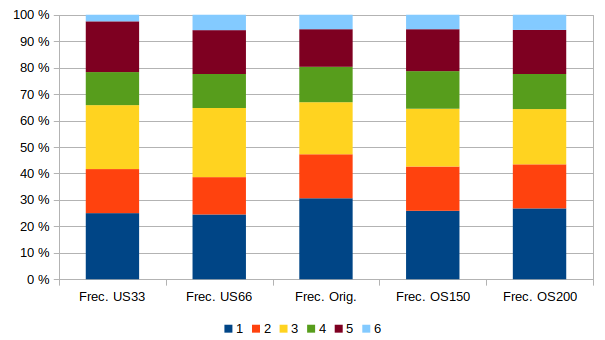
\includegraphics[scale=0.63]{supervised-resample-bias0-dist}
    \caption{Frecuencias de clases al hacer resample con \code{biasToUniformClass=0}}
    \label{fig:supervised-resample-bias0-dist}
\end{figure}

En la tabla \ref{tab:supervised-resample-bias1-dist} aparecen los datos de los distintos resamples realizados y se comparan las frecuencias de las clases con las originales. Estos datos se han obtenido con \code{biasToUniformClass=1}. En este caso, los porcentajes de patrones de cada clase tienden a igualarse, tal como se puede ver en el gráfico \ref{fig:supervised-resample-bias1-dist}.

\begin{table}[ht]
    \centering
    \begin{tabular}{|r|rr|rr|
    >{\columncolor[HTML]{C0C0C0}}r 
    >{\columncolor[HTML]{C0C0C0}}r |rr|rr|}
    \hline
    \multicolumn{1}{|c|}{Clase} &
      \multicolumn{2}{c|}{Frec. US33} &
      \multicolumn{2}{c|}{Frec. US66} &
      \multicolumn{2}{c|}{\cellcolor[HTML]{C0C0C0}Frec. Orig.} &
      \multicolumn{2}{c|}{Frec. OS150} &
      \multicolumn{2}{c|}{Frec. OS200} \\ \hline
    1     & 16  & 13,33\% & 43  & 17,84\% & 112 & 30,60\%  & 93  & 16,94\%  & 122 & 16,67\%  \\
    2     & 16  & 13,33\% & 30  & 12,45\% & 61  & 16,67\%  & 88  & 16,03\%  & 120 & 16,39\%  \\
    3     & 26  & 21,67\% & 40  & 16,60\% & 72  & 19,67\%  & 93  & 16,94\%  & 114 & 15,57\%  \\
    4     & 17  & 14,17\% & 36  & 14,94\% & 49  & 13,39\%  & 93  & 16,94\%  & 132 & 18,03\%  \\
    5     & 24  & 20,00\% & 48  & 19,92\% & 52  & 14,21\%  & 97  & 17,67\%  & 123 & 16,80\%  \\
    6     & 21  & 17,50\% & 44  & 18,26\% & 20  & 5,46\%   & 85  & 15,48\%  & 121 & 16,53\%  \\ \hline
    Total\footnote{Porcentajes respecto al tamaño muestral inicial} & 120 & 32,79\% & 241 & 65,85\% & 366 & 100,00\% & 549 & 150,00\% & 732 & 200,00\% \\ \hline
    \end{tabular}
    \caption{Frecuencias de clases con diferentes resamples y \code{biasToUniformClass=1}}
    \label{tab:supervised-resample-bias1-dist}
\end{table}
\begin{figure}[H]
    \centering
    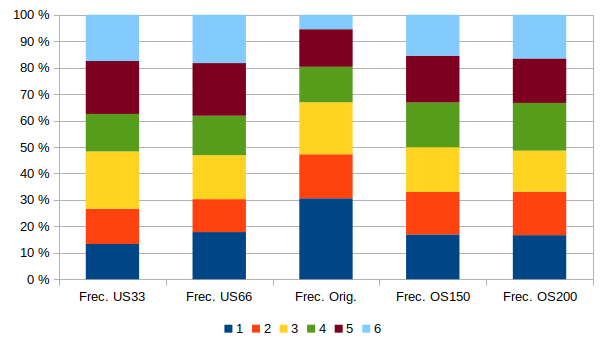
\includegraphics[scale=0.63]{supervised-resample-bias1-dist}
    \caption{Frecuencias de clases al hacer resamples con \code{biasToUniformClass=1}}
    \label{fig:supervised-resample-bias1-dist}
\end{figure}

\subsection{filters/supervised/instance/ClassBalancer}
\label{sec:supervised-class-balancer}
El filtro supervisado \code{ClassBalancer} asigna pesos ponderados a los patrones de manera que se equilibren las clases. Los patrones de una clase menos frecuente tendrán pesos ponderados mayores y viceversa, de manera que cada clase tenga en suma el mismo peso. En caso de que la clase fuese numérica, el filtro además la discretiza.

\begin{figure}[ht]
    \centering
    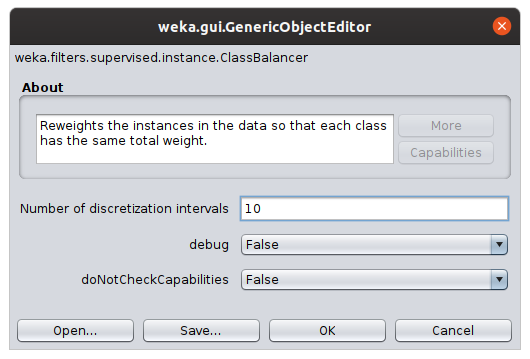
\includegraphics[scale=0.35]{supervised-class-balancer}
    \caption{Diálogo de configuración del filtro supervisado \code{ClassBalancer}}
    \label{fig:supervised-class-balancer}
\end{figure}

Los parámetros del filtro son los que aparecen en la figura \ref{fig:supervised-class-balancer} y se describen a continuación:
\begin{itemize}
    \item \code{Number of discretization intervals (10)}: Nº de intervalos que se establecen al discretizar la clase, en caso de que sea de tipo numérico.
    \item \code{debug False/True}: si se pone a true saca más información en el log al ejecutar el filtro.
    \item \code{doNotCheckCapabilities (False/True)}: habilita o deshabilita la comprobación de los datos. Afecta al rendimiento del filtro.
\end{itemize}

Para probar este filtro se compondrá una base de datos de ejemplo, desbalanceada y con clase continua, de forma que podamos observar a la vez todas las capacidades del filtro. Cuando se aplica el filtro, la primera diferencia que se observa es que el gráfico de distribución de valores de la clase cambia (figs. \ref{fig:supervised-class-balancer-unweighted} y \ref{fig:supervised-class-balancer-weighted}).

\begin{figure}[H]
    \centering
    \begin{minipage}{0.50\textwidth}
        \centering
        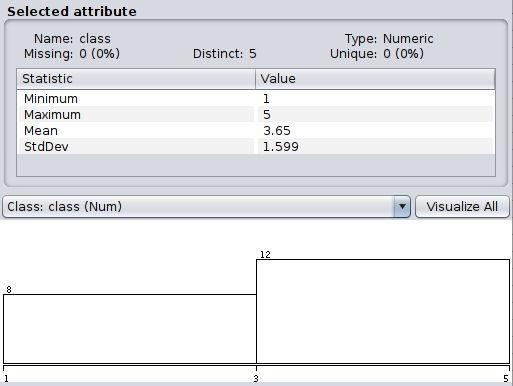
\includegraphics[scale=0.4]{supervised-class-balancer-unweighted}
        \caption{Datos de la clase antes de aplicar el filtro.}
        \label{fig:supervised-class-balancer-unweighted}
    \end{minipage}\hfill
    \begin{minipage}{0.50\textwidth}
        \centering
        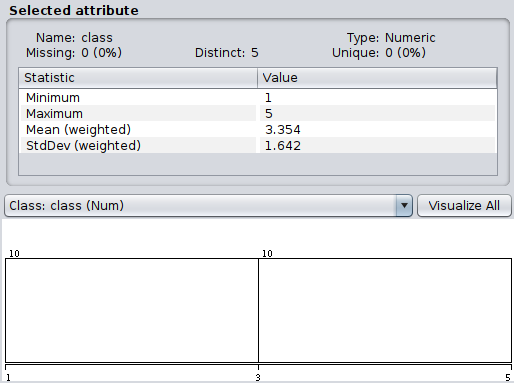
\includegraphics[scale=0.4]{supervised-class-balancer-weighted}
        \caption{Datos de la clase después de aplicar el filtro.}
        \label{fig:supervised-class-balancer-weighted}
    \end{minipage}
\end{figure}

Al aplicar el filtro, se ha añadido un nuevo campo llamado \code{Weight 1} con un valor numérico que representa el peso de la instancia para equilibrar la clase a la que pertenece. En la figura \ref{fig:supervised-class-balancer-int2} podemos ver cómo los pesos asignados balancean la clase en dos intervalos: $[1,3]$ y $(3,5]$. El primer intervalo tiene un peso de $0.8\overline{3}$ y tiene 12 patrones $0.8\overline{3}\cdot 12 = 10$. El segundo intervalo tiene un peso de $1.25$ y contiene 8 patrones: $1.25\cdot 8=10$. En la figura \ref{fig:supervised-class-balancer-int5} podemos ver cómo los pesos asignados balancean la clase en cinco grupos, tantos como valores diferentes toma la clase. A los $3$ patrones clase $1$ se les asigna peso $1.\overline{3}$, por lo que $1.\overline{3}\cdot 3 = 4$. A los 3 patrones con clase 2, les corresponde, obviamente, el mismo peso que a los de clase 1. A los 2 de clase 3, al igual que a los dos de clase 4, se les asigna peso $2$, resultando $2\cdot2=4$. Por último, a los $10$ patrones de clase 5 se les asigna peso $0.4$, lo que resulta en $0.4\cdot10=4$. Como se puede observar, todos los intervalos tienen el mismo peso.

\begin{figure}[H]
    \centering
    \begin{minipage}{0.50\textwidth}
        \centering
        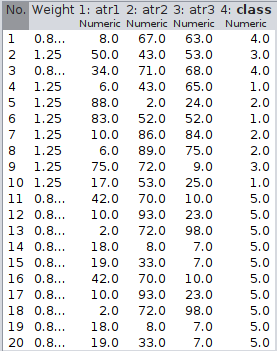
\includegraphics[scale=0.5]{supervised-class-balancer-int2}
        \caption{Datos balanceados en dos intervalos.}
        \label{fig:supervised-class-balancer-int2}
    \end{minipage}\hfill
    \begin{minipage}{0.50\textwidth}
        \centering
        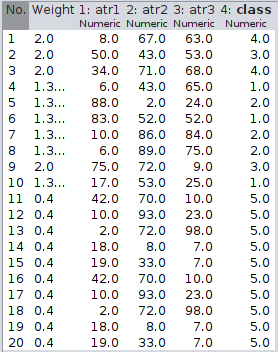
\includegraphics[scale=0.5]{supervised-class-balancer-int5}
        \caption{Datos balanceados en cinco intervalos.}
        \label{fig:supervised-class-balancer-int5}
    \end{minipage}
\end{figure}

\subsection{filters/supervised/instance/SpreadSubsample}
El filtro supervisado \code{SpreadSubsample} realiza remuestreos balanceados de la base de datos. Es decir, produce un nuevo conjunto a partir del anterior con un determinado balance de frecuencias de las clases.


\begin{figure}[H]
    \centering
    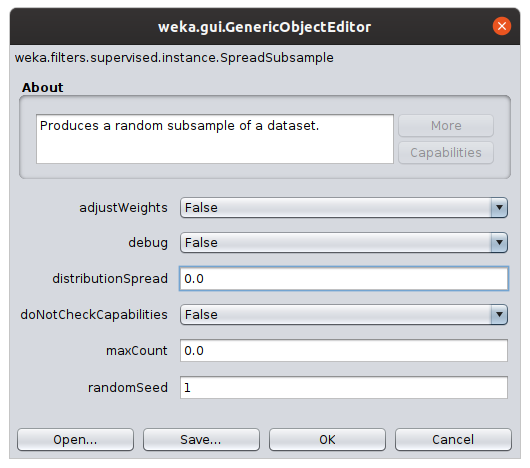
\includegraphics[scale=0.4]{supervised-spread-subsample}
    \caption{Configuración del filtro supervisado \code{SpreadSubsample}.}
    \label{fig:supervised-spread-subsample}
\end{figure}

Como se puede observar en la fig. \ref{fig:supervised-spread-subsample}, el filtro \code{SpreadSubsample} cuenta con los siguientes parámetros:
\begin{itemize}
    \item \code{adjustWeights (False/True)}: si se pone a true, añade a la base de datos el campo \code{Weight} y le asigna un peso ponderado para mantener el mismo equilibro entre clases que hubiera antes de aplicar el filtro (ver \ref{sec:supervised-class-balancer}).
    \item \code{debug (False/True)}: si se pone a true saca más información en el log al ejecutar el filtro.
    \item \code{distributionSpread (num)}: 0 para no establecer proporción máxima, $n | 10\geq n\geq 1$ para permitir un desequilibro máximo entre clases clases de $n:1$.
    \item \code{doNotCheckCapabilities (False/True)}: habilita o deshabilita la comprobación de los datos. Afecta al rendimiento del filtro.
    \item \code{maxCount (num)}: establece un límite máximo de patrones por clase. 0 para desactivar esta función.
    \item \code{randomSeed (num)}: semilla para la selección aleatoria.
\end{itemize}

Para probar este filtro se utiliza la base de datos \code{breast-cancer} por ser su clase binaria y con una distribución 201-85 (fig. \ref{fig:supervised-spread-subsample-breast-cancer}). En una primera prueba, con los parámetros por defecto, no se ha visto ningún cambio en la base de datos al aplicar el filtro. El primer cambio introducido ha sido el valor 50 en el parámetro \code{maxCount}, lo que ha producido subsampling que ha igualado el nº de patrones de cada clase a 50 (fig. \ref{fig:supervised-spread-subsample-max50}).


\begin{figure}[H]
    \centering
    \begin{minipage}{0.50\textwidth}
        \centering
        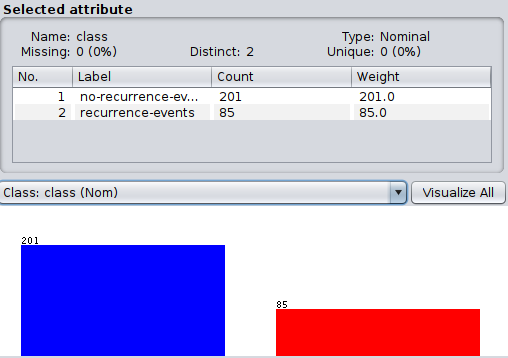
\includegraphics[scale=0.40 ]{supervised-spread-subsample-breast-cancer}
        \caption{Distribución inicial de la clase en la base de datos \code{breast-cancer}.}
        \label{fig:supervised-spread-subsample-breast-cancer}
    \end{minipage}\hfill
    \begin{minipage}{0.50\textwidth}
        \centering
        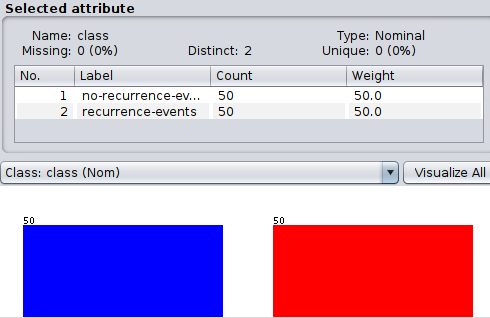
\includegraphics[scale=0.44]{supervised-spread-subsample-max50}
        \caption{Resultado del filtro con distributionSpread=0 y maxCount=50.}
        \label{fig:supervised-spread-subsample-max50}
    \end{minipage}
\end{figure}

La segunda prueba ha consistido en fijar de nuevo \code{maxCount} a 0 y \code{distributionSpread}a 1. Esta configuración sirve para que la proporción máxima entre las clases sea $1:1$, así que también equilibra la distribución de las clases, eliminando patrones de la clase mayoritaria hasta quedar tantos como tenga la minoritaria (fig. \ref{fig:supervised-spread-subsample-spr1}). Por último, se establece \code{distributionSpread} a 1.5 con el fin de obtener una proporción $3:2$. Deberíamos tener 3 patrones de la clase \code{no-recurrence-events} por cada dos de la clase \code{recurrence-events}. Una vez aplicado el filtro con la configuración indicada (fig. \ref{fig:supervised-spread-subsample-spr1.5}), vemos que el resultado es el esperado: 127 frente a 85 patrones de cada clase.

\begin{figure}[H]
    \centering
    \begin{minipage}{0.50\textwidth}
        \centering
        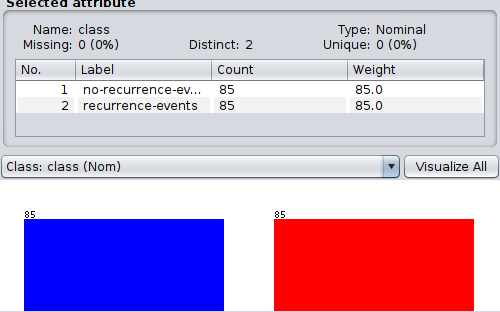
\includegraphics[scale=0.44]{supervised-spread-subsample-spr1}
        \caption{Resultado del filtro con distributionSpread=1 y maxCount=0.}
        \label{fig:supervised-spread-subsample-spr1}
    \end{minipage}\hfill
    \begin{minipage}{0.50\textwidth}
        \centering
        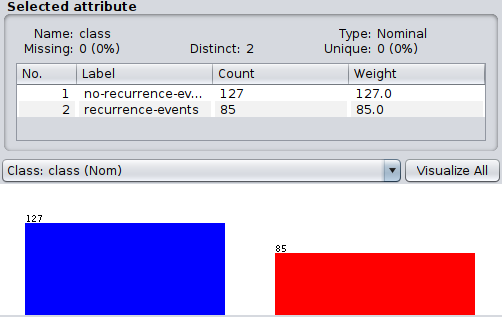
\includegraphics[scale=0.45]{supervised-spread-subsample-spr15}
        \caption{Resultado del filtro con distributionSpread=1.5.}
        \label{fig:supervised-spread-subsample-spr1.5}
    \end{minipage}
\end{figure}